\section{Render Loop}
\label{chapter:design:loop}

	The communication between PURGE and the external \classname{Renderer} is heavily dependent on the render loop -- or main loop -- of our library. The loop basically consists of three different stages that need to be run through repeatedly:

	\begin{numlist}
		\item gathering user input,
		\item updating the scene and
		\item rendering the scene.
	\end{numlist}

	We will be using the ``Single-thread Uncoupled model'' presented by \cite{Valente_Conci_Feijo_2005}, which cycles through these stations periodically in a single thread and updates the objects using the time elapsed since the last cycle. We will see in Section \ref{chapter:implementation:loop}, that the choice of the implementation does not have a strong impact on the API.

	The render loop in a graphics engine must provide an API for the repeated modification of the scene by the application. The sequence described above (gather input, update, render) is present in all reference engines, but each of them approaches this problem quite differently:

	\begin{biglist}
		\item Ogre3d: Provides the FrameListener interface\footnote{http://www.ogre3d.org/docs/api/html/classOgre\_1\_1FrameListener.html} for the registration of recurring tasks during the loop cycle. Developers can implement this interface to react to certain events in the rendering loop, usually the end of the render cycle. The current version provides three such events:

		\begin{smalllist}
			\item \inlinecode{frameStarted()}: Called before the frame is being rendered.
			\item \inlinecode{frameRenderingQueued()}: Called while the GPU is computing the current frame. This event is useful in the case one wants to make use of the CPU at this time, as the CPU would otherwise be idle and the application would block until the GPU is finished.
			\item \inlinecode{frameEnded()}: Called after the rendering is finished.
		\end{smalllist}

		Ogre3d does not have native routines for processing input from external devices (such as keyboards or mice), but an external project is recommended for this purpose throughout the documentation: OIS\footnote{The official web-site of the project is http://www.wreckedgames.com, but more information can be found on its sourceforge project site: http://sourceforge.net/projects/wgois/}. This external library again provides two methods of processing input: buffered and unbuffered. If the library is used in buffered mode, all input can be processed at once during the execution of a frame listener. In unbuffered mode, a listener has to be provided to the library that will be called immediately on the retrieval of new events through system interrupts.

		\item Panda3d: Allows the registration of tasks to be continuously performed at a central facility, the \classname{AsyncTaskManager}. As the name suggests, the library is capable of distributing ongoing tasks across different threads and actually makes use of this mechanism to manage the rendering loop. The rendering step itself is nothing more than a \classname{GenericAsyncTask}. A nice option is the registration of function pointers instead of full-blown classes, which makes playing around with the library a bit more convenient.

		The \classname{AsyncTaskManager} holds multiple instances of \classname{AsyncTaskChain}, which contain objects of type \classname{AsyncTask}. Each \classname{AsyncTaskChain} can run in a separate thread. Furthermore, each \classname{AsyncTask} has a sort number that ensures that tasks can be executed in a predefined order across all \classname{AsyncTaskChain}s. Figure \ref{fig:PandaTasks} visualizes the sequence in a single cycle with two \classname{AsyncTaskChain}s.

		Unfortunately, the name \classname{Chain} is a bit misleading in this context. The name suggests a linear dependence between ``links'', which is not the case: The ``links'' in the chain have additional dependencies to other links in other chains, as seen in Figure \ref{fig:PandaTasks}. A more accurate visual representation of this approach would possibly be ``thread'', reminding of the computational thread it possibly runs in and the thread of a woven fabric, having dependences to other threads.

		\begin{figure}[htbp]
			\centering
			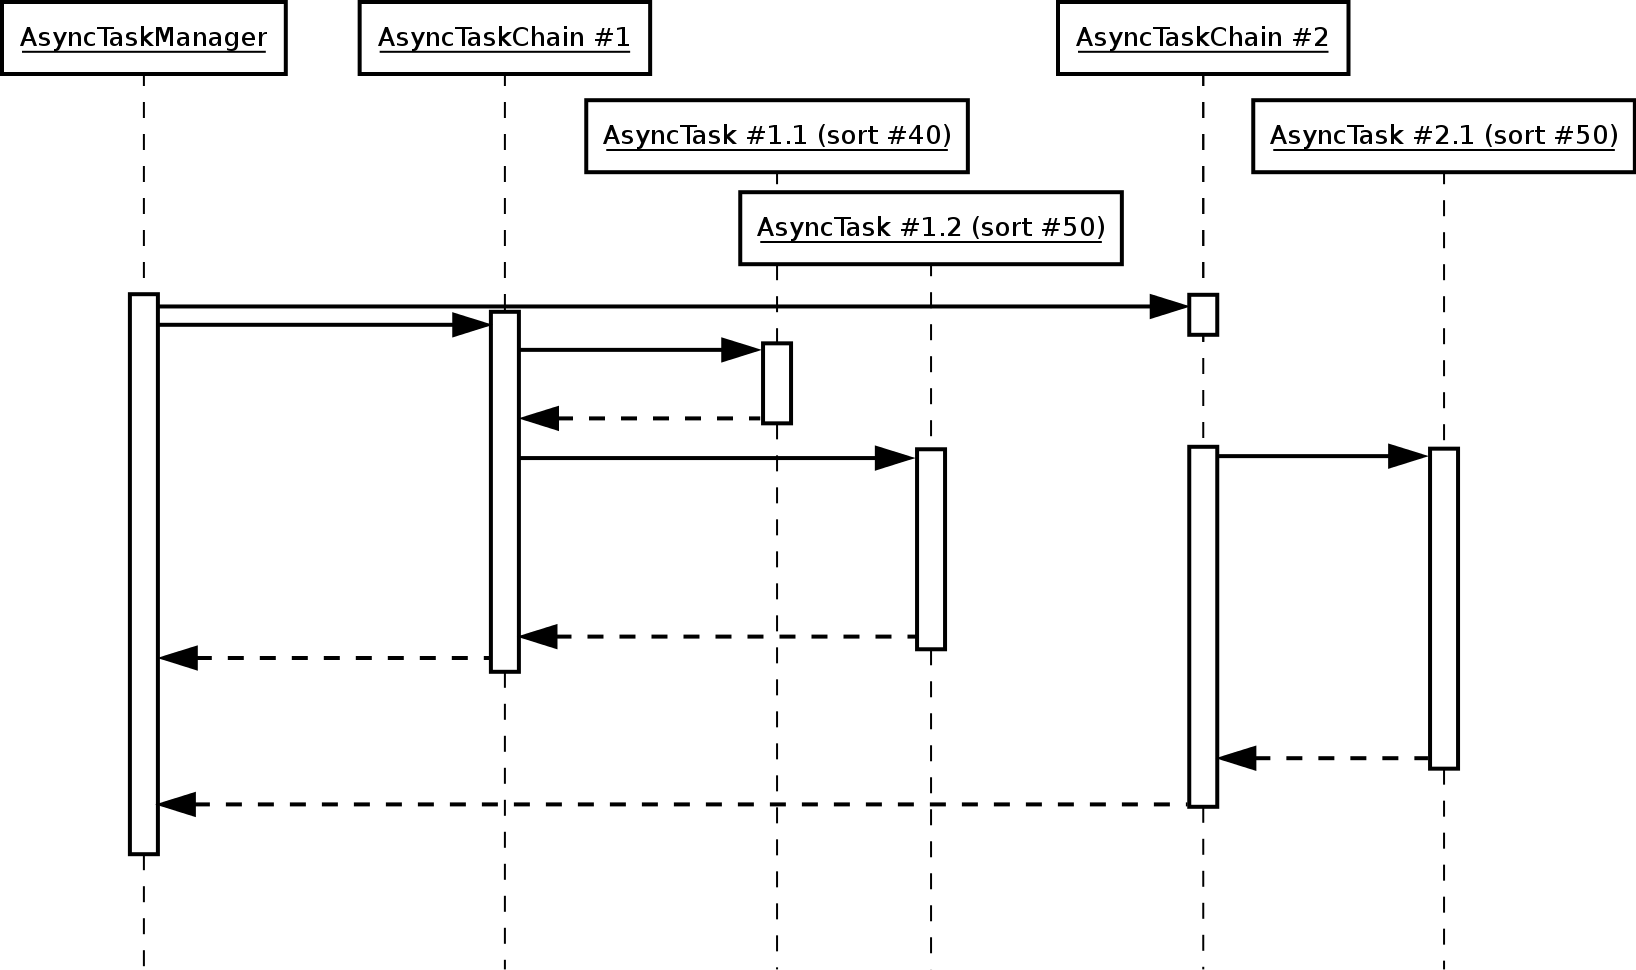
\includegraphics[width=14cm]{images/PandaTasks.png}
			\caption{Simplified sequence diagram of a single rendering cycle in Panda3d. \inlinecode{AsyncTaskChain \#1} and \inlinecode{AsyncTaskChain \#2} start running simultaneously, but the second chain will block until the first task in the first chain was executed, as it has a smaller sort value than the task in the second chain.}
			\label{fig:PandaTasks}
		\end{figure}

		\item OpenSceneGraph: As the project does not provide a render loop \emph{per se}, it is possible to implement ones own loop that takes care of any operations in-between the rendered frames.
			
			But another peculiarity of OpenSceneGraph is the strong focus on the scene graph, even when designing the application flow. We had seen that the scene graph is actually a data structure for organizing objects in space. OpenSceneGraph additionally allows the registration of callbacks to scene nodes. These \classname{NodeCallback}s\footnote{http://www.openscenegraph.org/documentation/NPSTutorials/osgFollowMe.htm} are called during the rendering process as part of the render loop that updates the scene graph.
		
	\end{biglist}

	Among the analyzed libraries, Panda3d provides the most flexible API for managing the scene during the main loop. It allows us to split the loop into multiple threads, making good use of multiple CPUs, but the API emphasizes an early decision which tasks could be performed in separate threads. It requires the definition of \classname{AsyncTaskChain}s for the integration of new tasks into the loop. A dependence between the tasks is then established through the so-called sort numbers.

	An alternative implementation could hide away the details of threading just by introducing Task groups as outlined in Figure \ref{fig:Task}. A Task group adopts the duty of the numeric sort number in Panda3d's loop design. Instead of assigning a value to a task, it is instead added to the same task group as other tasks that can be processed simultaneously.
	
	\begin{figure}[htbp]
		\centering
		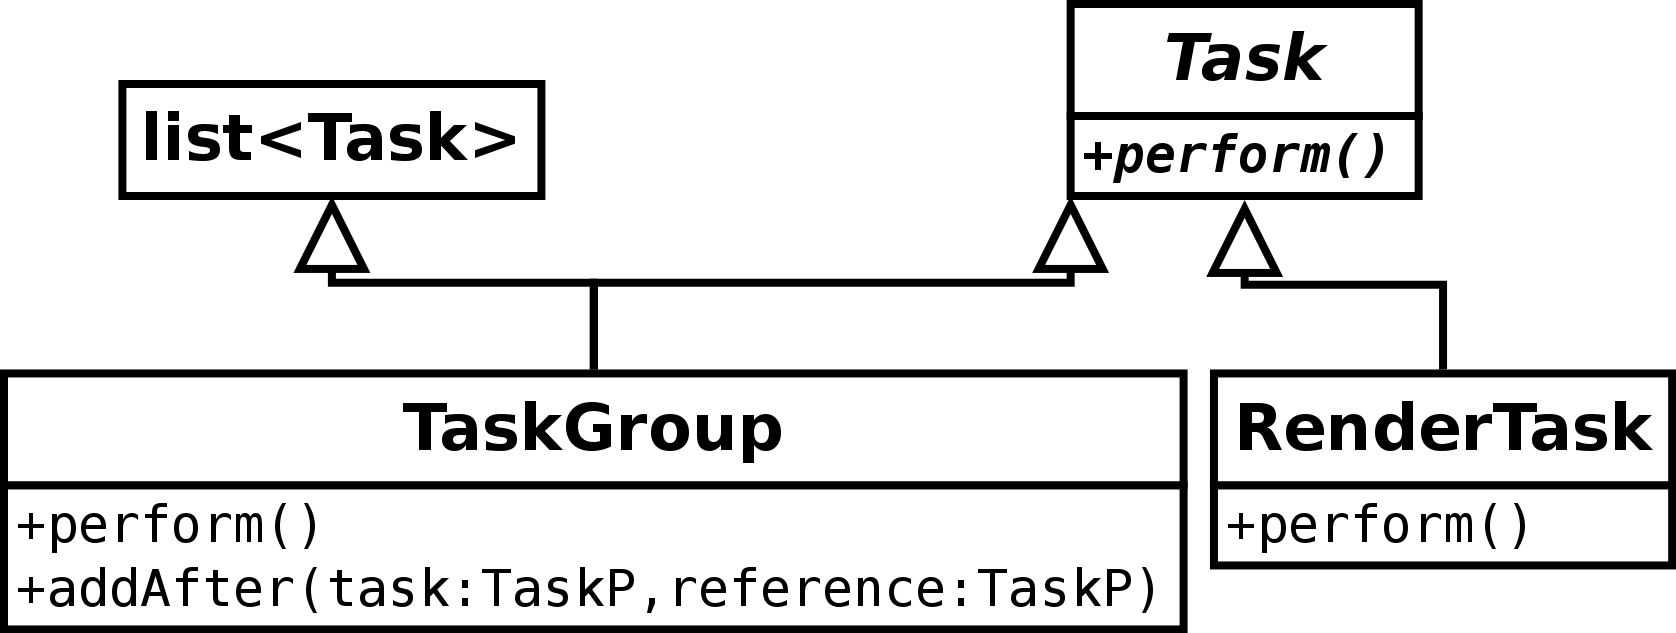
\includegraphics[width=10cm]{images/Task.png}
		\caption{\classname{Task} and \classname{TaskGroup} class hierarchy.}
		\label{fig:Task}
	\end{figure}

	This implementation is in contrast to Panda3d's implementation choice, as it does not group tasks by their ability to run in parallel, but rather creates groups of tasks that need to be performed sequentially -- handling input, computing Physics, computing AI choices, updating positions, and rendering are some examples of such task groups.

	The design described above is equivalent to having a single flat rendering loop that executes tasks sequentially. The \classname{TaskGroup} structure is introduced for convenient re-arranging of the loop elements as a tree structure. With an adequate \classname{TaskGroup} re-implementation it would be further possible to insert parallelism into this design. Although this implementation is not accomplished within this thesis, we will look at it briefly in Section \ref{chapter:implementation:loop}.

	To further simplify the process of adding Tasks to a task group, we will add additional functions to the \classname{TaskGroup} class. These functions will further improve the usability by reducing the number of calls necessary to perform common operations: Adding a task after another reference task, for example.

	While looking into the implementation of the communication between PURGE and the \classname{Renderer} in Section \ref{chapter:implementation:renderer}, we will further discuss the single mandatory task of the library: the \classname{RenderTask}.

